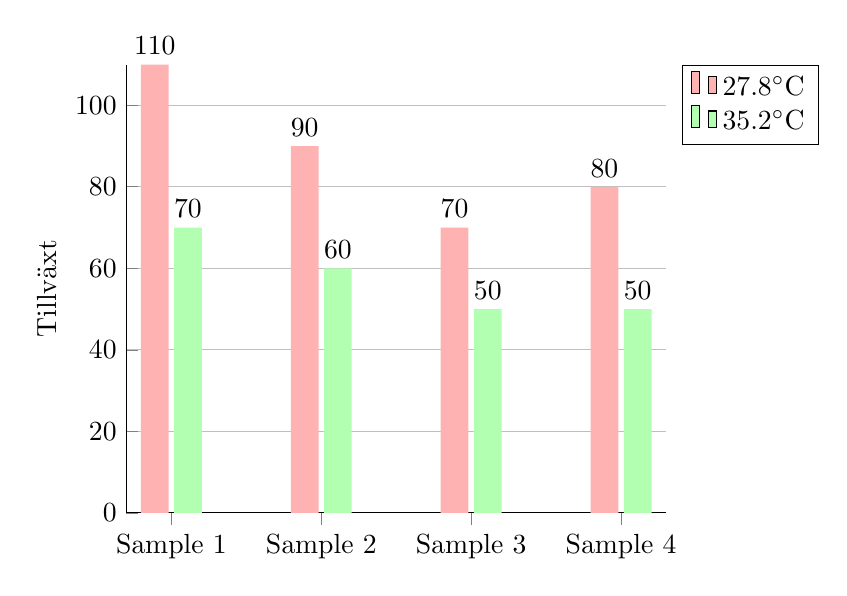
\begin{tikzpicture}
	\begin{axis}[
			ybar,
			ymin=0, ymax=110,
			axis lines*=left,
			ylabel={Tillväxt},
			symbolic x coords={Sample 1, Sample 2, Sample 3, Sample 4},
			xtick=data,
			legend entries={$27.8^\circ$C, $35.2^\circ$C},
			legend pos=outer north east,
			ymajorgrids=true,
			nodes near coords={\pgfmathprintnumber[precision=0]{\pgfplotspointmeta}}
		]
		\addplot [draw=none,fill=red!30] coordinates {
			(Sample 1, 110)
			(Sample 2, 90)
			(Sample 3, 70)
			(Sample 4, 80)
		};

		\addplot [draw=none, fill=green!30] coordinates {
			(Sample 1, 70)
			(Sample 2, 60)
			(Sample 3, 50)
			(Sample 4, 50)
		};
	\end{axis}
\end{tikzpicture}
